\section{Brainstorm UI}
\label{prototype:BrainstormUI}
After considering the feedback I gained from my primary research and my learnings from my research of Ui design techniques I began planning out the layout for my web application.

First I began planning out my 'user flows' these are the intents my user may have when entering the website and I am aiming to minimise the friction they will face whilst completing their goals

User Flows:
\begin{enumerate}
    \item Exploring List of notes -> opening a few notes and reading around
    \item Quickly taking notes -> organising these loose notes
    \item Searching for a specific note 
    \item Searching for specific information (may be among multiple pages)
    \item Managing user account details
\end{enumerate}

Next I thought about the various UI elements these flows would require

\begin{tabularx}{\textwidth}{>{\raggedright\arraybackslash}X>{\raggedright\arraybackslash}X}
    \rowcolor{gray!15} \textbf{Flow}           & \textbf{Required UI}                           \\
    1   & Graphical view of information, able to edit notes after opening, multiple pages per tab\\
    2  & Quick note view, dashboard component on application launch, \\
    3 & note search bar, filters within graph view\\
    4 & Global search bar, quick switching between pages\\
    5 & Global settings menu, customizable interface options\\
\end{tabularx}

Now i took to paper and sketched some initial ideas:
\begin{figure}[H]
    \centering
    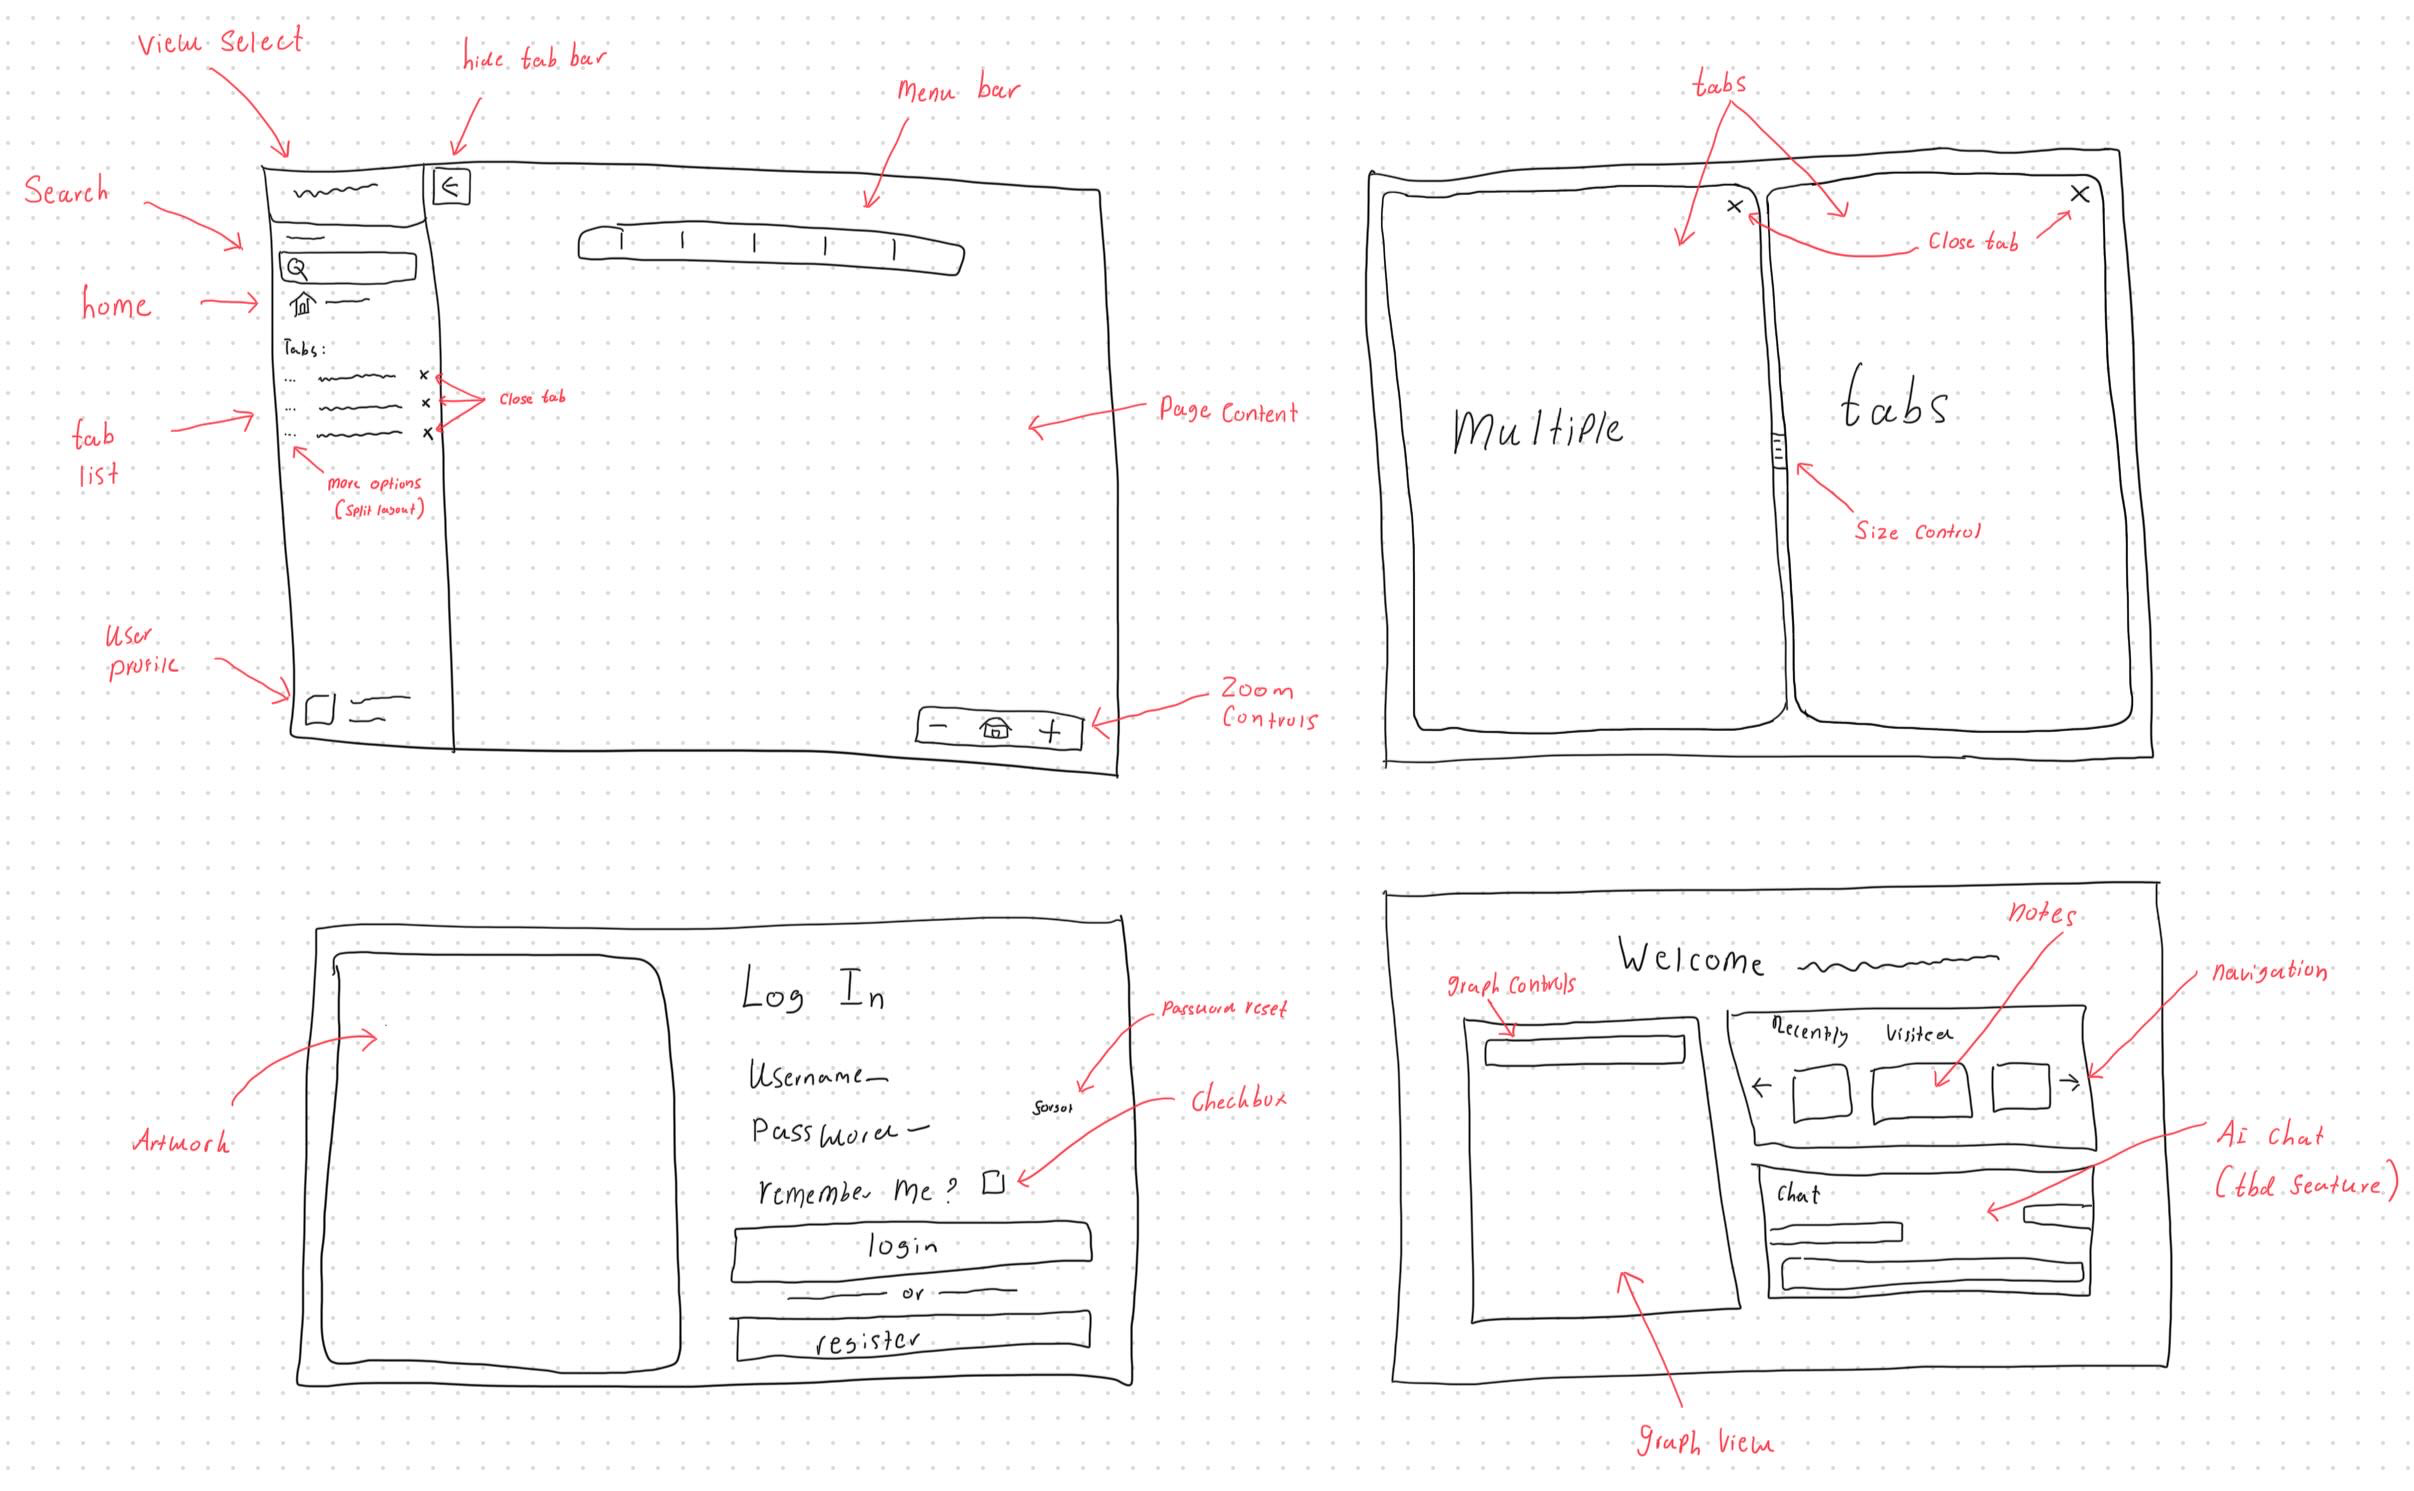
\includegraphics[width=0.8\textwidth]{Prototype/16_BrainstormUI/media/initialSketches.png}
    \caption{Initial Sketches UI design}
    \label{fig:brainstormUI}
\end{figure}

Fairly happy with these primative shapes i then moved to Figma to create a more polished version of my ideas. I had previously researched Figma and its capabilities as a prototyping tool and was excited to get started with it. I had also seen the power of component libraries in Figma which would allow me to quickly prototype my ideas without having to create every element from scratch.

\begin{figure}[H]
    \centering
    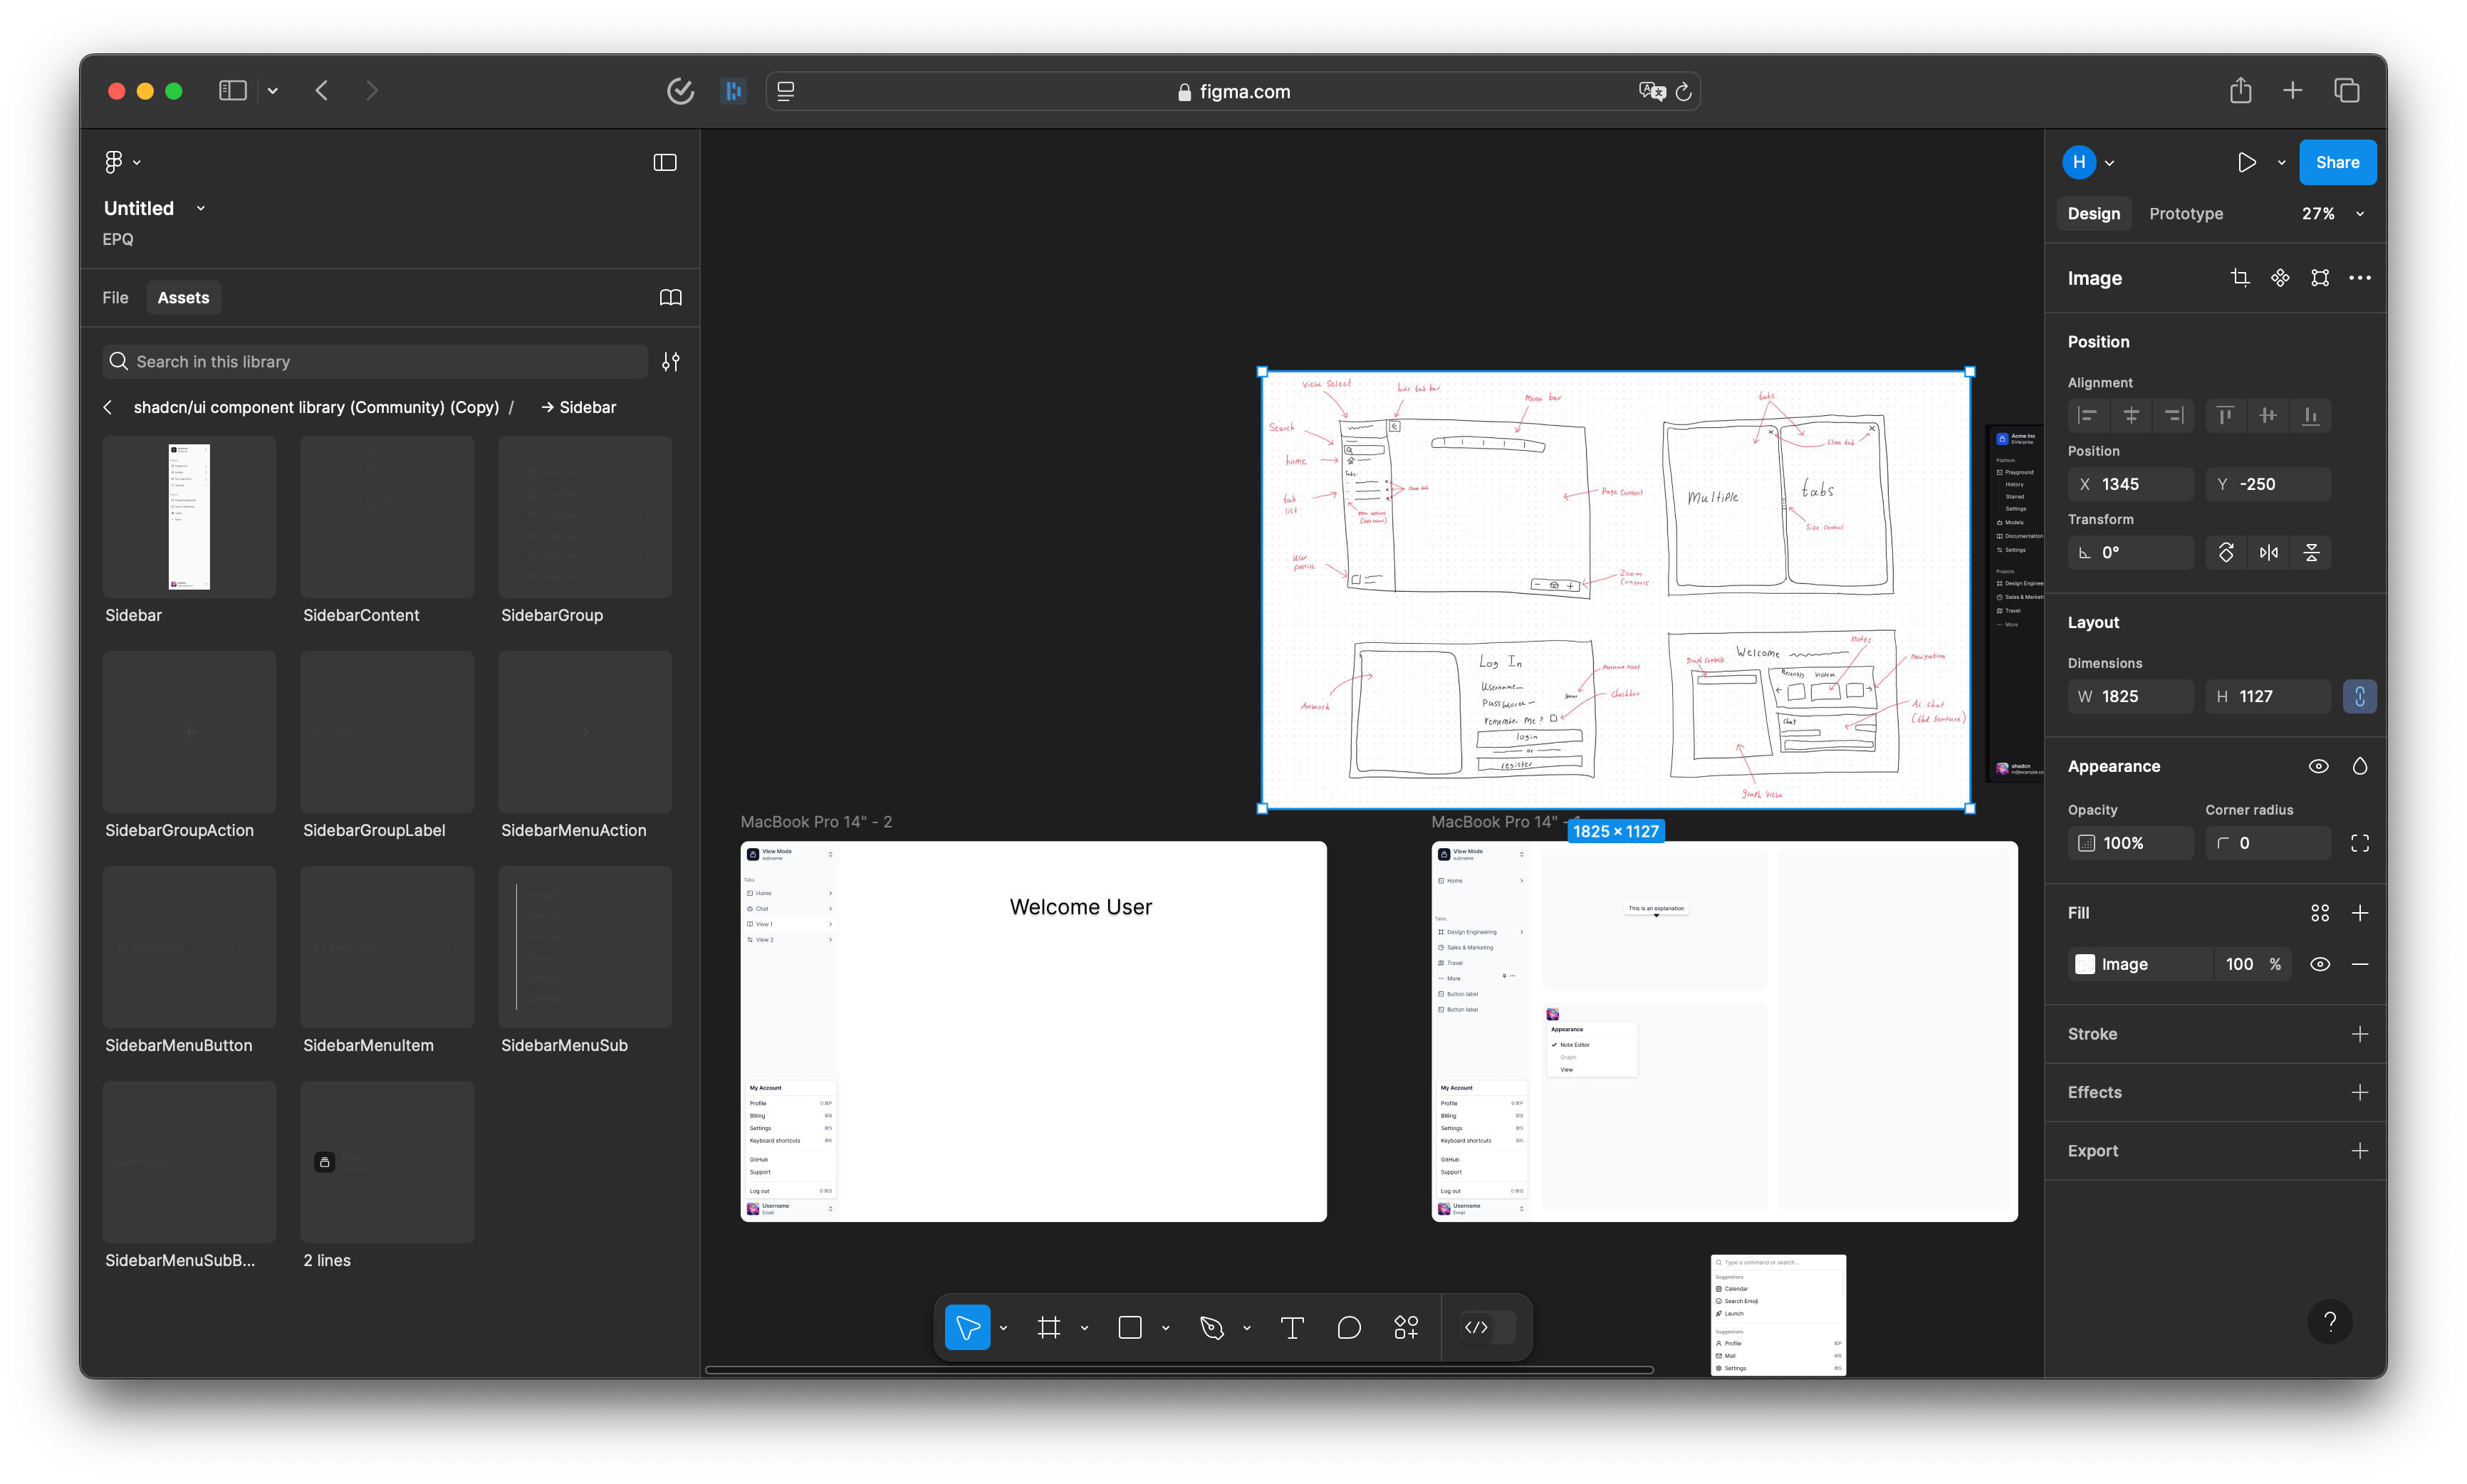
\includegraphics[width=0.8\textwidth]{Prototype/16_BrainstormUI/media/figmaSketch.png}
    \caption{Figma UI Design}
    \label{fig:brainstormUIFigma}
\end{figure}

The final iteration used a Shadcn component library within Figma to finalise some ideas as the user would see them, this helped me to produce a sidebar that made tab management and feature access simple for users.

\begin{figure}[H]
    \centering
    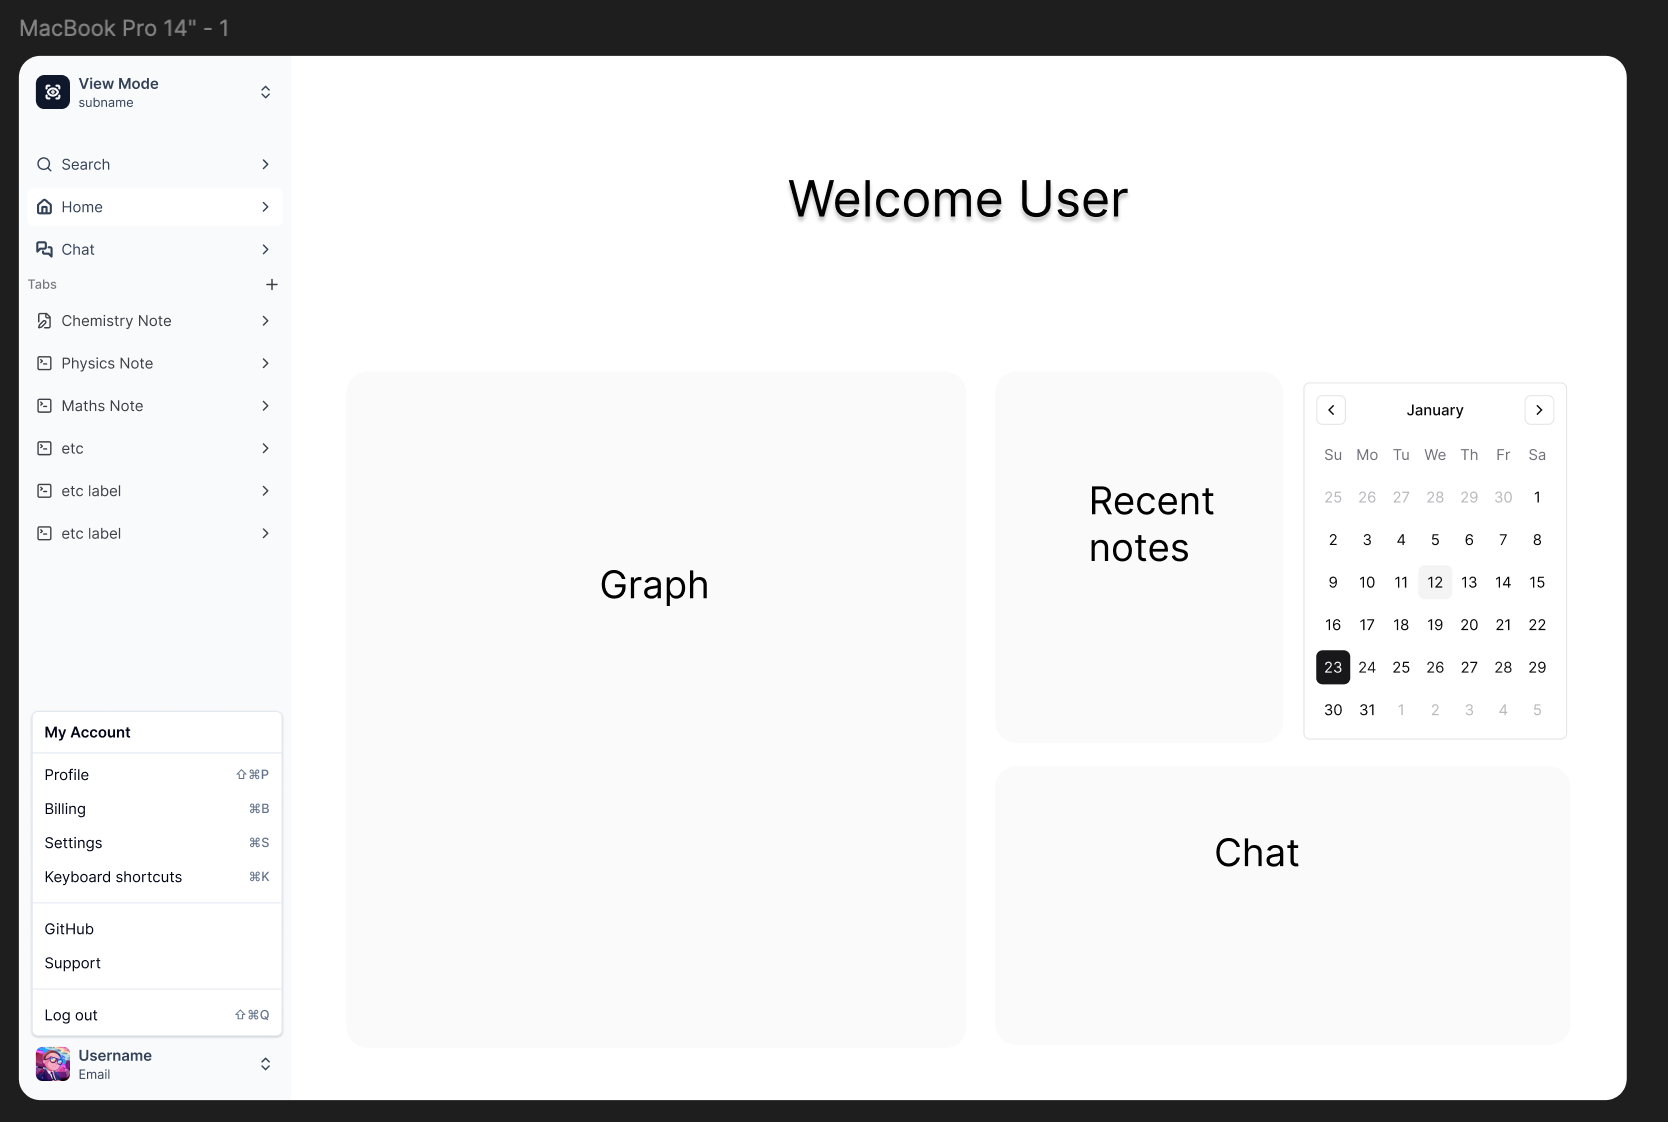
\includegraphics[width=0.8\textwidth]{Prototype/16_BrainstormUI/media/figmaFinal.png}
    \caption{Final Figma UI Design}
    \label{fig:brainstormUIFinal}
\end{figure}